\documentclass[14pt]{beamer}

% Presento style file
\usepackage{config/presento}
\usepackage{graphicx}

\graphicspath{ {images/} }

% custom command and packages
\input{config/custom-command}

% Information
\title{PHPUnit}
\subtitle{The PHP Testing Framework}
\author{Sitdhibong Laokok}
\institute{Computer Engineering}
\date{\today}

\begin{document}

% Title page
\begin{frame}[plain]
\maketitle
\end{frame}

\begin{frame}[plain]{Outline}
    \tableofcontents
\end{frame}

\section{Overview}
\begin{frame}[plain]{Why you should Test?}
    \begin{fullpageitemize}
        \item<1-> Increase confidence in change/maintaining code 
        \item<2-> Code more reuseable 
        \item<3-> Development is fast
        \item<4-> Less of \textcolor{red}{CODE DEBT}
        \item<5-> Debuging is easy
        \item<6-> Code are more reliable
    \end{fullpageitemize}
\end{frame}

\begin{frame}[plain]{Manual test}
    \begin{figure}
        \center
        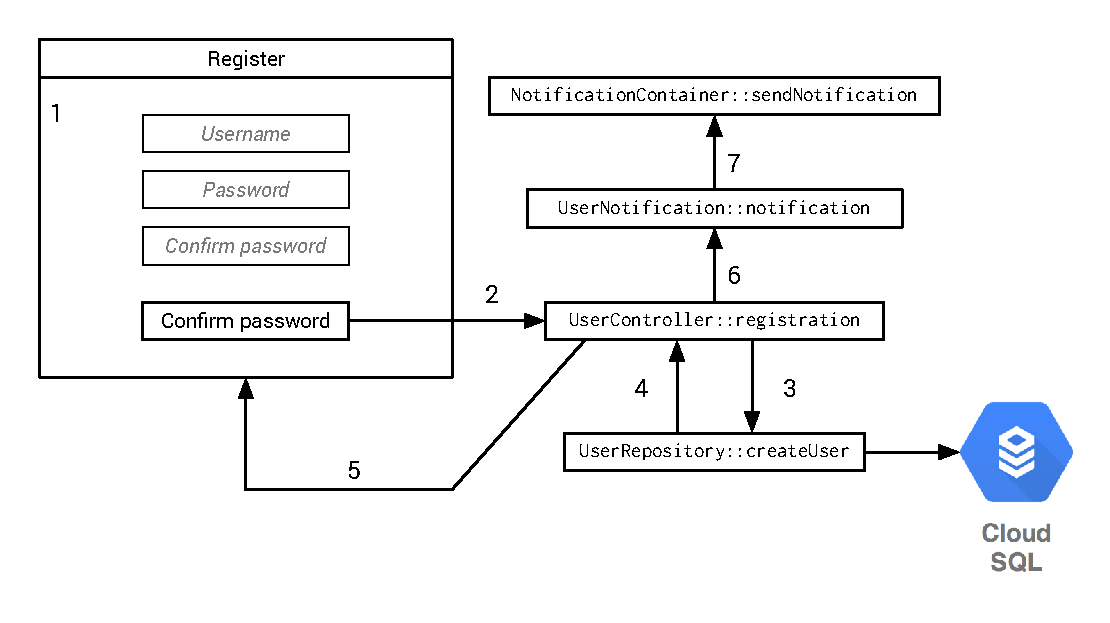
\includegraphics[width=\textwidth]{normal-test}
    \end{figure}
\end{frame}

\begin{frame}[plain]{V-Model}
    \begin{figure}
        \center
        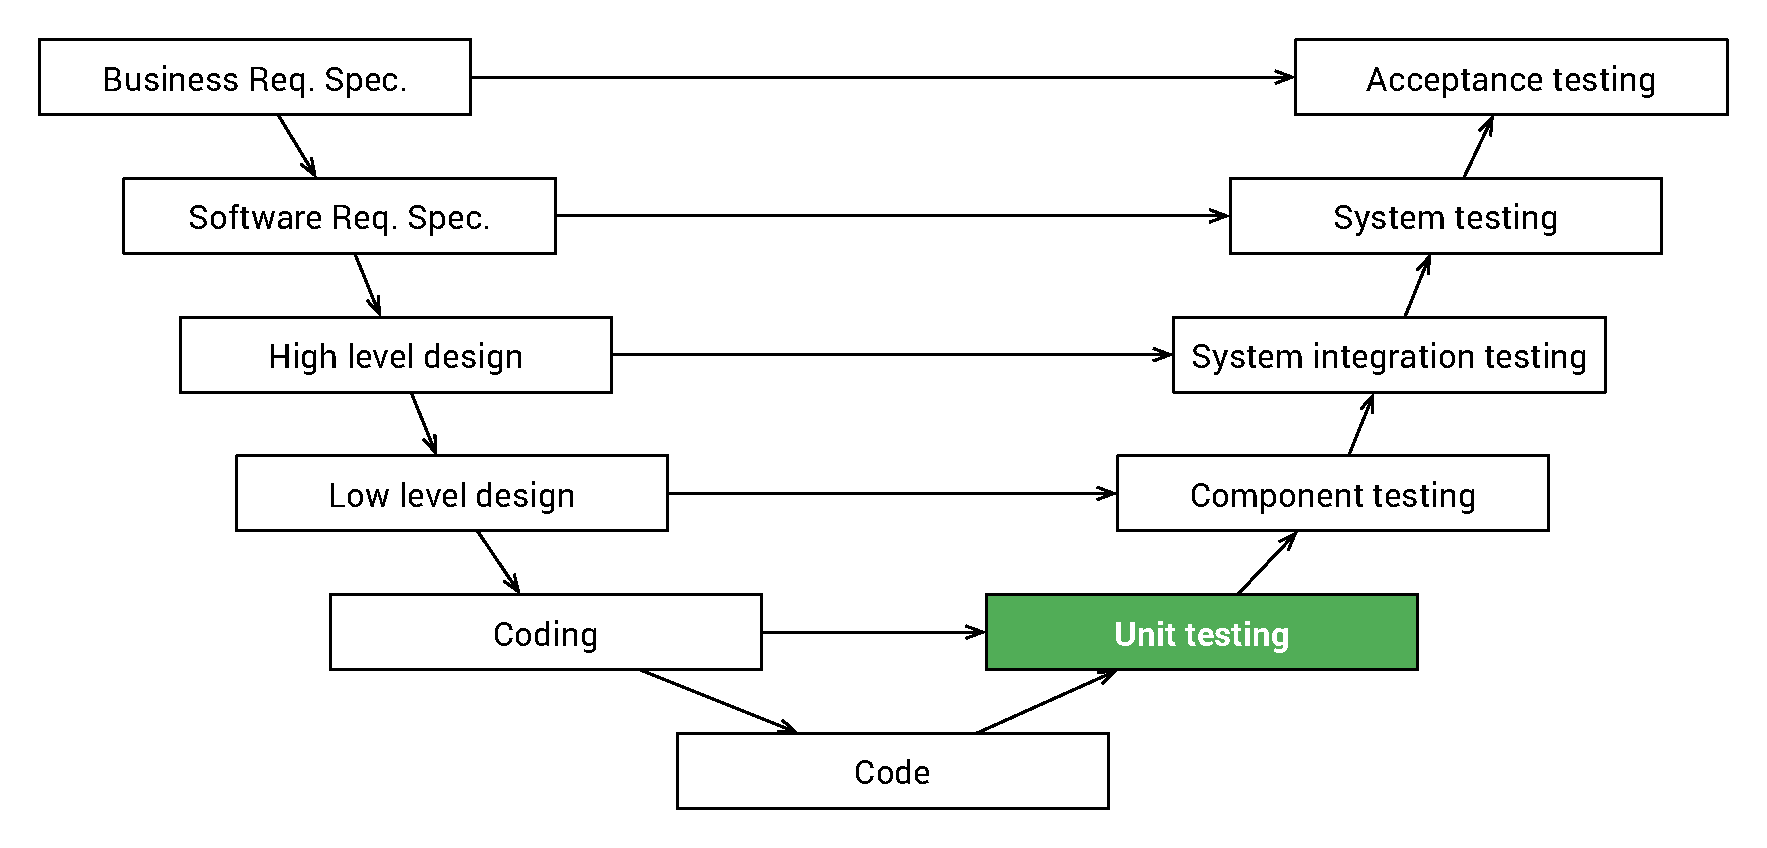
\includegraphics[width=\textwidth]{v-model}
    \end{figure}
\end{frame}

\begin{frame}[plain]{Key qualities of a good unit test}
    \begin{fullpageitemize}
        \item<1-> Environment free
        \item<2-> One at a time
        \item<3-> No side effect
        \item<4-> Assert the results
        \item<5-> Fast
    \end{fullpageitemize}
    % https://www.kenneth-truyers.net/2012/12/15/key-qualities-of-a-good-unit-test/
\end{frame}

\begin{frame}[plain]{Unit test mantra}
    \begin{figure}
        \center
        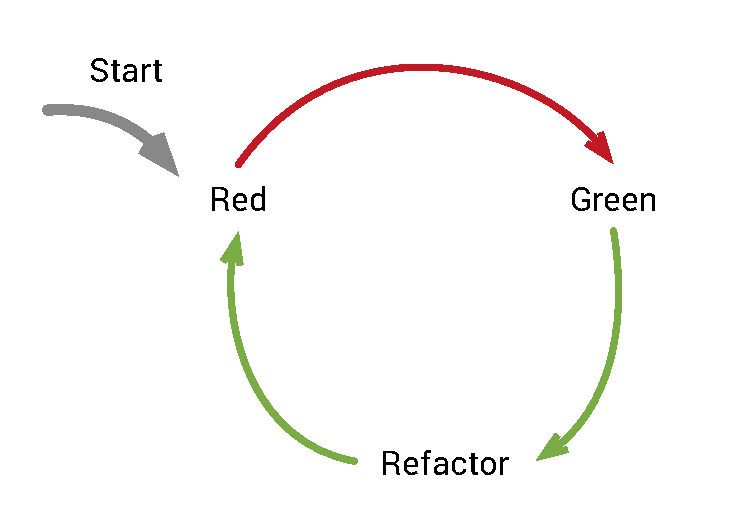
\includegraphics[width=.9\textwidth]{failng-pass-refactor}
        \label{fig:failng-pass-refactor}
    \end{figure}
\end{frame}

\begin{frame}[plain]{Driver \& Stub}
    \begin{figure}
        \center
        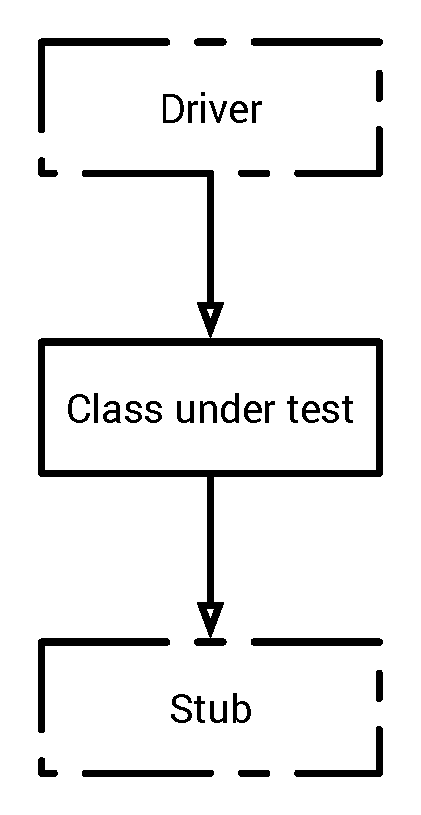
\includegraphics[height=.8\textheight]{driver-and-stub}
        \label{fig:driver-and-stub}
    \end{figure}
\end{frame}

\section{Writing Test Case}
\begin{frame}[plain]{Core techniques}
    \begin{fullpageitemize}
        \item Using stubs to break dependencies
        \item Interation testing using mock objects
    \end{fullpageitemize}
\end{frame}

\begin{frame}[plain]{The pillars of good unit tests}
    \begin{fullpageitemize}
        \item Writing trustworthy tests
        \item Writing maintainable tests
        \item Writing readable tests
    \end{fullpageitemize}
\end{frame}

\begin{frame}[plain]{Fixture}
    \begin{fullpageitemize}
        \item<1-> \color{colororange}{\inconsolatafont{setUpBeforeClass()}}
        \item<2-> \color{colorhgray}{Test Class}
        \item<3-> \color{colororange}{\inconsolatafont{setUp()}}
        \item<4-> \color{colorhgray}{Test cases}
        \item<5-> \color{colororange}{\inconsolatafont{tearDown()}}
        \item<6-> \color{colorhgray}{Final test case}
        \item<7-> \color{colororange}{\inconsolatafont{tearDownAfterClass()}}
    \end{fullpageitemize}
\end{frame}

\begin{frame}[plain]{Test Case's Structure}
    \begin{fullpageitemize}
        \item<1-> \em{\textcolor{gray}{Given}} \\
            Set up \\

        \item<2-> \em{\textcolor{gray}{When}} \\
            Do something \\

        \item<3-> \em{\textcolor{gray}{Then}} \\
            assert
    \end{fullpageitemize}
\end{frame}

\begin{frame}[plain]{Assert}
    \hugetext{\[expected \iff actual\]}
\end{frame}

\begin{frame}[plain]{Assert}
    \Large{
        \inconsolatafont{ 
        assert{\textcolor{red}{*}}(\$expected, \\
        ~~~~\$actual, \\
        ~~~~\em{"Description"})
        }
    }
\end{frame}

\begin{frame}[plain]{Assert - Example}
    \Large{
        \inconsolatafont{ 
        assert{\textcolor{red}{*}}(\$expected, \\
        ~~~~\$actual, \\
        ~~~~\em{"Description"})
        }
    }
\end{frame}

\section{Coding}
\framecard[colororange]{{\color{white}\hugetext{Coding}}}

\begin{frame}[plain]{High Level Design: Deployment}
    \begin{figure}
        \center
        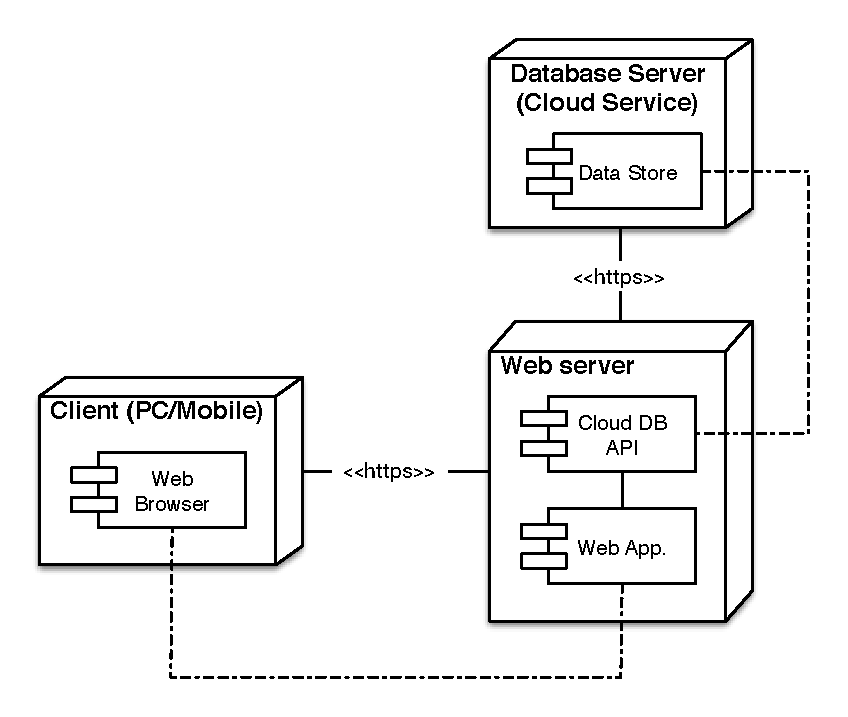
\includegraphics[width=0.7\textwidth]{deployment-grading-system}
        \label{fig:deployment-grading-system}
    \end{figure}
\end{frame}

\begin{frame}[plain]{Low Level Design: Class diagram}
    \begin{figure}
        \center
        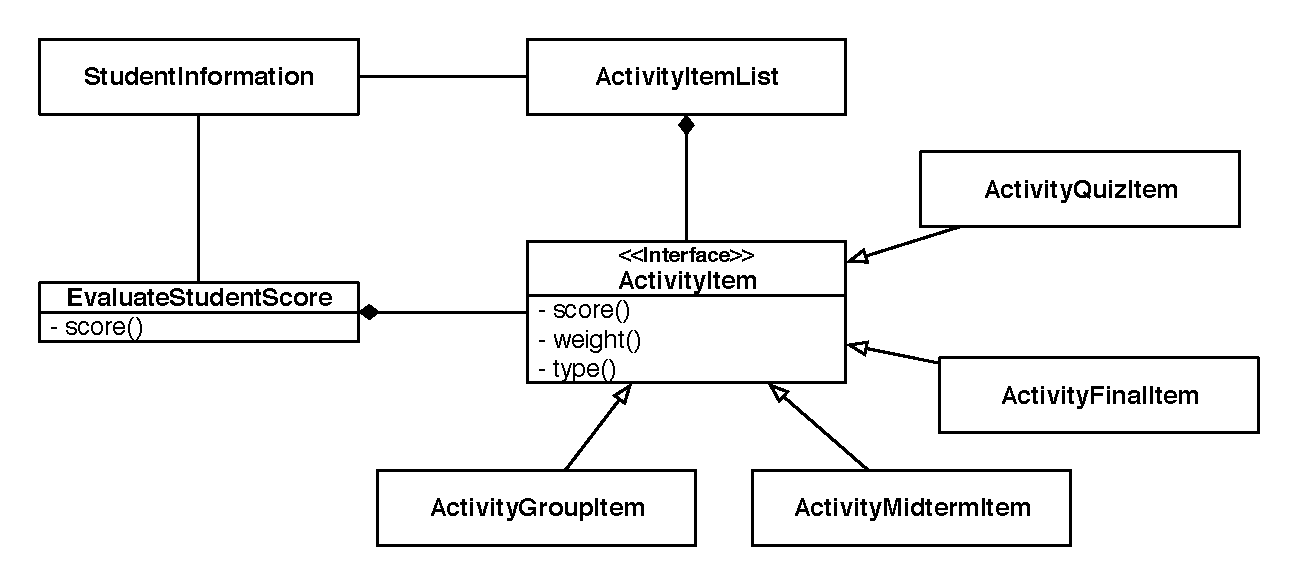
\includegraphics[width=\textwidth]{class-diagram}
        \label{fig:class-diagram}
    \end{figure}
\end{frame}

% sections in the presentation
% \begin{frame}{Presento}
%     \begin{fullpageitemize}
%         \item \begin{center}\largetext{The design is \underline{clean}}\end{center}
%         \item \begin{center}\largetext{The rules are \underline{simple}}\end{center}
%         \item \begin{center}\largetext{The code is \underline{extensible}}\end{center}
%     \end{fullpageitemize}
% \end{frame}
% 
% \begin{frame}{Open Source Fonts}
%     \begin{fullpageitemize}
%         \item {\montserratfont This is Montserrat}
%         \item {\notosansfont This is Noto Sans}
%         \item {\latolightfont This is Lato (light)}
%         \item {\inconsolatafont This is inconsolata}
%         \item \textsc{This is Alegreya Sans small caps}
%     \end{fullpageitemize}
% \end{frame}
% 
% \begin{frame}{Color Palette}
%     \begin{center}
%         \crule[colordgray] \crule[colorhgray] \crule[colorblue] \crule[colorgreen] \crule[colororange]
%     \end{center}
% \end{frame}
% 
% \framecard[colorgreen]{{\color{white}\hugetext{BIG BOLD TEXT}}}
 
% \framepic[0.8]{images/skeleton}{
%  \begin{textblock}{7}(7,2.5)
%     {\color{colorblue}\hugetext{\textbf{RUN!}}}
%  \end{textblock}
% }

\begin{frame}[plain]{Books}
    \begin{figure}
        \center
        \includegraphics[height=.7\textheight]{TDD-by-Example}
        \label{fig:TDD-by-Example}
    \end{figure}
\end{frame}

\begin{frame}[plain]{Books}
    \begin{figure}
        \center
        \includegraphics[height=.7\textheight]{TDD-with-Python}
        \label{fig:TDD-with-Python}
    \end{figure}
\end{frame}

\begin{frame}[plain]{Books}
    \begin{figure}
        \center
        \includegraphics[height=.7\textheight]{the-art-of-unit-testing}
        \label{fig:the-art-of-unit-testing}
    \end{figure}
\end{frame}

\end{document}
